\section{Discretization}

Computing truly event-based optical flow is challenging from a computational point of view. 
It would require the algorithm to evaluate how each discrete event contributes to the flow field created by all other events in a given, possibly infinite, time span.
We make the following simplifications.
Firstly, we discretize the spatio-temporal Gabor filter in time with a given time step and in space with the resolution equal to that of the DVS camera.
We choose the spatio-temporal span of the filter as the volume in which the magnitude of the filter's response does not fall below some threshold value.
The filter thus comprises of discrete time-slices, which we call Filter Slices (FS).
Secondly, all events occurring in a single time window are grouped together or quantized into the so-called Event Slice (ES) and are assumed to have occurred at the same moment, \emph{i.e.} the beginning of the current time step. 
An ES is a (sparse) matrix, with the number of entries equal to that of the DVS camera and their value being the sum of events which occurred at a given location. 
With this setup, computing optical flow means filtering the incoming stream of Event Slices with the precomputed Gabor filter.


\subsection{Computational Pipeline}
A natural approach is to streamline the work, setting several components up in a computational pipeline.
Data comes into the pipeline and is processed sequentially by each of the components, leaving as a final product or optical flow field in our case. 
Typically, data has to be read and post-processed.
This gives the final shape to our pipeline, as shown in Figure \ref{fig:pipeline}, which consists of EventReader, Quantizer, FilteringEngine and FlowSink objects.

\begin{figure}[ht!]
 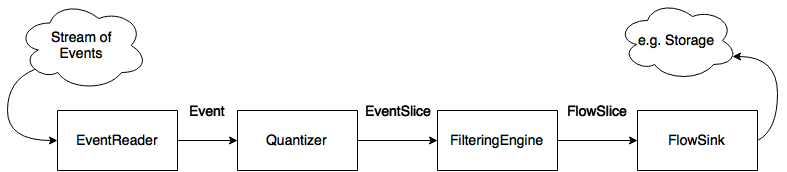
\includegraphics[width=\textwidth]{figs/pipeline}
 \caption{Pipeline}
  \label{fig:pipeline}
\end{figure}

EventReader reads an event stream from different sources, \emph{e.g.,} text file, binary file or directly from a DVS camera.
Events are passed to the Quantizer, which quantizes discrete events into Event Slices.
They are consumed by the FilteringEngine. It has an internal buffer, which holds enough events to cover the whole time span of the filter. 
Once the buffer fills up, FilteringEngine starts producing Flow Slices.
The FlowSink object handles them by either serializing or visualizing the resulting optical flow field.

\subsection{Filtering Engine}

% introduction
Filtering in the spatio-temporal domain is applied to the data by convolving it linearly with the filter.
The filter, discretized as above, as well as Event Slices corresponding to the filter's time span can be seen as big 3-dimensional matrices.
It is well known that once the matrices' sizes are big enough, filtering in spatio-temporal domain can be prohibitively expensive.
We could either exploit sparse structure of Event Slices or transform the problem to the frequency domain, where spatio-temporal convolution corresponds to element-wise multiplication of the filter with data.
We decided to go with the the 2\textsuperscript{nd} approach.
\\

% why series of 2D convolutions
Possibly the most efficient way to carry out convolution would be to aggregate enough Event Slices, apply 3D Fourier transform, multiply it with the transformed filter element-wise and apply the 3D inverse transform to the result.
There are 2 limiting factors, however.
Firstly, linear convolution requires padding both the filter and data to the same size, in 1D given by $M+N-1$ where $M$ -- filter dimension and $N$ -- data dimension.
It significantly increases the amount of elements to process, the more the higher the dimensionality.
Secondly, at every time step (for every incoming Event Slice) the process of padding and applying 3D Fourier transform would have to be repeated.
Each ES would have to be transformed as many times as many Filter Slices there are.
Therefore, we decided to use 2-dimensional Fourier transforms, which enable vast reuse of values computed in previous iterations of the algorithm.
3-dimensional convolution can be expressed as a sum of 2-dimensional ones.
Each Event Slice still has to be convolved with all Filter Slices, but it can be transformed to the frequency domain only once and reused later.

\begin{algorithm}
 \caption{Filtering Algorithm}
 \label{algo:optic}
 \begin{algorithmic}[1]
  \Procedure{Filter}{eventSlice}
  \State rotate(eventSliceBuffer)
  \State pad(eventSlice)  
  \State slice(eventSliceBuffer, 0) = forwardFourier2D(eventSlice)
  \State flow = 0
  \For{each filter $\in$ filters }
  \State response = 0
  \For{each $i \in$ numSlices(filter) }
  \State filterSlice = slice(filter, $i$)
  \State eventSlice = slice(eventSliceBuffer, $i$)
  \State response += filterSlice $\cdot$ eventSlice
  \EndFor
  \State flow.X += cos(angle(filter)) $\cdot$ response
  \State flow.Y -= sin(angle(filter)) $\cdot$ response
  \EndFor
  \State inverseFourier2D(flow.X)
  \State inverseFourier2D(flow.Y)
  \State return flow
  \EndProcedure
\end{algorithmic}

\end{algorithm}